\documentclass[12pt, a4paper]{article}
\usepackage{listings}
\usepackage{xcolor}
\usepackage{pdfpages}
\usepackage{amsmath}
\usepackage{amssymb}
\usepackage{gensymb}
\usepackage{wrapfig}
\usepackage{graphicx}
\usepackage{blindtext}
\usepackage{subcaption}
\usepackage[export]{adjustbox}
\usepackage{blindtext}
\usepackage{multicol}
\usepackage{appendix}
\usepackage{float}
\usepackage[style=authoryear]{biblatex}
\usepackage{titling}
\usepackage[hidelinks=true]{hyperref}
\usepackage[inner=15mm, outer=15mm, top=15mm, bottom=20mm]{geometry}
\usepackage[T1]{fontenc}
\usepackage[normalem]{ulem}
\usepackage{multirow}
\usepackage{titlesec}
\usepackage{booktabs, array, tabularx}
\usepackage{xcolor}
\usepackage{wasysym}
\usepackage{tocloft}
\usepackage{tikz}
\usepackage[list=true]{subcaption}
\usepackage[bottom]{footmisc}


\definecolor{dkgreen}{rgb}{0,0.6,0}
\definecolor{mauve}{rgb}{0.58,0,0.82}

\bibliography{DFM_References}

\lstdefinestyle{C++}{
  language=C++,
  numbers=none,
  stepnumber=1,
  basicstyle=\scriptsize\ttfamily,
  numbersep=10pt,
  tabsize=4,
  showspaces=false,
  showstringspaces=false,
  keywordstyle=\color{blue},
  commentstyle=\color{dkgreen},
  stringstyle=\color{mauve},
  breaklines=true,
  postbreak=\mbox{\textcolor{red}{$\hookrightarrow$}\space}
}
\lstset{style=C++}

\newcommand{\reqref}[1]{Section \ref{sec:requirements}:\ref{#1}}
\newcommand{\CITATION}{{\color{red}(CITATION NEEDED)}}
\newcommand{\TODO}[1]{{\color{red}\textbf{TODO} #1}}

\newcommand{\email}[1]{
  \small{\textit{\href{mailto:#1}{#1}}}
}

\title{
  \huge\textbf{MXEN 2002} \\
  \vspace{2em}
  \large\textbf{Project Report}\\
  \vspace{0.5em}
}

\preauthor{
  \vspace{12cm}
  \begin{center}
    \begin{tabular}[t]{c}
}

\author{
    \textbf{Kee-An Seet} \\
    \email{19776219@student.curtin.edu.au} \\
    \textbf{Harry Cassidy} \\
    \email{20607591@student.curtin.edu.au}
}

\postauthor{
    \end{tabular}
    \par
  \end{center}
}

\newcommand{\listequationsname}{\Large \hspace{3mm} List of Equations}
\newlistof{myequations}{equ}{\listequationsname}
\newcommand{\myequations}[1]{%
\addcontentsline{equ}{myequations}{\hspace{8mm}\protect\numberline{\hspace{-2mm}\theequation}#1}\par}


\date{}

\begin{document}
\pagenumbering{gobble}
\maketitle
\pagebreak

\pagenumbering{roman}
\tableofcontents
\paragraph{}
\newpage
\listoffigures
\paragraph{}
\listoftables
\listofmyequations
\paragraph{}
\pagebreak

\pagenumbering{arabic}

\section{Nomenclature}\label{sec:nomen}
\paragraph{}
\begin{table}[h]
    \centering
    \begin{tabular}{l|l}
      Symbol & Description~ \\ \hline \hline
      A & Cross-sectional area (mm2) \\ \hline
      c & Maximum distance from the centroid to outer perimeter (mm)      \\ \hline                          
    \end{tabular}
    \caption{Nomenclature}
    \label{tab:nome}
  \end{table}

\newpage
\section{The Task} \label{sec:intro}

\paragraph{}
  We were tasked with building, wiring, and programming a robot to complete a series of objectives, such as navigating a maze autonomously and moving a camera with a servo as to let the operator identify targets. We were to use the Arduino Mega hardware with a DC motor drive system along with several distance sensors to help achieve the objectives.

\begin{figure}[h]
  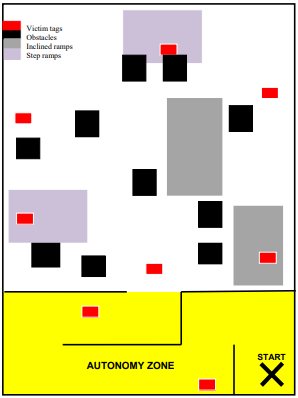
\includegraphics{Images/AutonZone.png}
  \centering
  \caption{Supplied example of the task map}
  \label{fig:intro:map}
\end{figure}

\subsection{Autonomy Zone}
  \paragraph{}
    The "Autonomy Zone" is the section of the map in which the robot is completely self controlled. The idea behind this challenge is that in the event of a connection dsiruption in a dangerous area for humans, the robot should be able to rescue it's self from danger.

\subsection{Manual Control}
 \paragraph{}
    The majority of the task is to control the robot through wireless communication. During this period the robot (controlled by the user) must drive through the zone and send a camera feed back to the user for "victim" tags to be recorded.


\newpage

\section{Our Solution} \label{sec:Solution}
\subsection{Joystick Drive}
  \paragraph{}
    To be able to control the robot manually, we implemented a joystick drive system, where joystick inputs on the controller would result in movement of the robot. Since the raw joystick outputs have a range from 0-1024, they were first scaled by a factor of 1/4 (to bring it within 0-256 range) and then transmitted to the robot via the XBees.
    These values were processed on the robot's end by mapping them from 0 - 256 to -378 - 378, which were used to calculate 2 variables, leftValue and rightValue, where $leftValue = joyY + joyX$ and $rightValue = joyY - joyX$.
    This achieves a differential drive effect, where both left and right motors react to the joystick Y position for forwards and backwards drive, but each react in opposite magntidues depending on the joystick X position, resulting in the turning of the robot.
  \paragraph{}
    To convert these drive values into values that can run the motors, we opted for a PWM drive system, where PWM signals are used to control the speed of each DC motor independently.
\subsection{PWM Calculations}
  \paragraph{}
    We aimed to have our duty cycle range between 0.05s and 0.1s.
    A Phase Correct PWM mode was chosen as it allowed for the widest range of possible values and prescaler values.
    We also settled on prescaler value of 8 as it allowed the resulting COMP value to be within the 0-10000 range that the ADC can read at.

    Phase Correct PWM: f(base) = f(microcontroller)/(2*TOP*PRE)

    TOP = 10000, PRE = 8

    $f(base) = (16*10^6) / (2*20000*8) = 50Hz$
    
    $Period = 0.02s$

    $Duty Cycle range: 0.05s - 0.1s$

    $Duty Cycle = COMP/TOP$

    $COMP range: (20000*0.05)-(20000*0.01) = 1000-2000$

    With this information we can choose which bits to set the PWM registers to. Our drivetrain used the TCCR1A and TCCR1B registers.

    As we decided to use PWM Phase correct (mode 10), we set the WGM11 and WGM13 bits in the PWM registers to 1. This mode meant that our TOP value of 20000 would be set in the ICR1 register.
    We want the PWM to clear on up count and compare on down count, so we set the COM1B1 bit to 1.
    Our prescaler is 8 which corresponds to setting only the CS11 bit to 1.

    The following table shows the bits set in the TCCR1A and TCCR1B PWM registers that control the drivetrain:
  \begin{table}[h]
    \centering
    \begin{tabular}{l|l|l|l|l|l|l|l|l}
      Register & COM1A1 & COM1A0 & COM1B1 & COM1B0 & COM1C1 & COM1C0 & WGM11 & WGM10 \\ \hline \hline
      TCCR1A & 1 & 0 & 1 & 0 & 0 & 0 & 1 & 0 \\ \hline                        
    \end{tabular}
    \caption{TCCR1A register}
    \label{tab:nome}
  \end{table}

  \begin{table}[h]
    \centering
    \begin{tabular}{l|l|l|l|l|l|l|l|l}
      Register & ICNC1 & ICES1 & - & WGM13 & WGM12 & CS12 & CS11 & CS10 \\ \hline \hline
      TCCR1A & 0 & 0 & 0 & 1 & 0 & 0 & 1 & 0 \\ \hline                        
    \end{tabular}
    \caption{TCCR1B register}
    \label{tab:nome}
  \end{table}

  \newpage

  \section{Program logic flowcharts} \label{sec:Flowchart}
  \subsection{Robot.c program logic}
  \begin{figure}[h]
    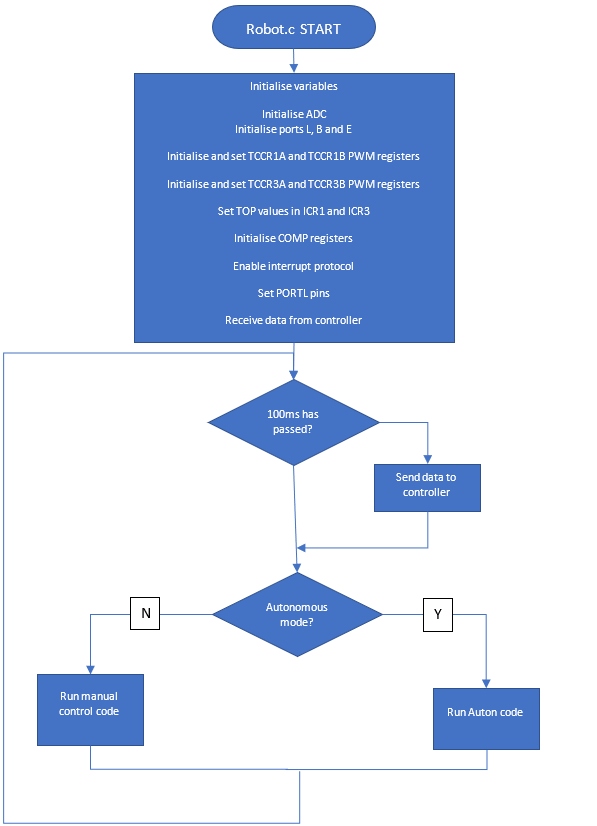
\includegraphics[width=0.7\columnwidth]{Images/robot_c.png}
    \centering
    \caption{Flowchart of Robot.c code}
    \label{fig:Flowchart:robot_c}
  \end{figure}

  \subsection{Autonomous code program logic}
  \begin{figure}[h]
    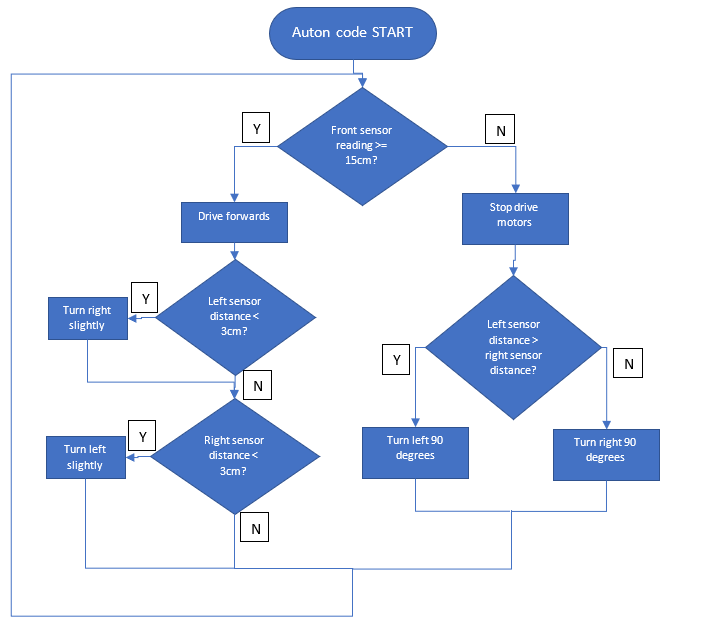
\includegraphics[width=0.9\columnwidth]{Images/auton.png}
    \centering
    \caption{Flowchart of autonomous mode code}
    \label{fig:Flowchart:auton}
  \end{figure}
  
\end{document}